\documentclass[aps,prl,reprint,amsmath,amssymb,floatfix,notitlepage]{revtex4-1}
%\documentclass[journal=ancac3,layout=twocolumn,manuscript=article]{achemso}

\newcommand*\mycommand[1]{\texttt{\emph{#1}}}
%\newcommand*{\INTERNAL}{}
\usepackage{chemformula} % Formula subscripts using \ch{}
\usepackage[T1]{fontenc} % Use modern font encodings
\usepackage{graphicx}% Include figure files
\usepackage{dcolumn}% Align table columns on decimal point
\usepackage{bm}% bold math
\usepackage{hyperref}% add hypertext capabilities
%\hypersetup{colorlinks=true,urlcolor={blue},citecolor={blue}, linkcolor={blue}}
\usepackage{amsmath} % or simply amstext
%\newcommand{\angstrom}{\textup{\angstrom}}
\usepackage{siunitx}
\usepackage{color}
\usepackage[normalem]{ulem}
\usepackage{diagbox}
\usepackage{import}
\usepackage{multirow}
\usepackage{xr} % referencing across multiple files
\usepackage{cleveref} % cite figures in SI

\renewcommand{\figurename}{Supporting Figure}
\renewcommand{\tablename}{Supporting Table}
\renewcommand{\thefigure}{S\arabic{figure}}
\renewcommand{\thetable}{S\arabic{table}}

\newcommand{\sinfo}{Supporting Information}

\newcommand{\lock}{\color{black}}
\newcommand{\zhzh}{\color{blue}}

% Use main text labels
\externaldocument[main-]{main}

\begin{document}

\title{\sinfo\ for \\
Adatoms in the Surface-Confined Ullmann Coupling of Phenyl Groups}% Force line breaks with \\
%\thanks{A footnote to the article title}%

\author{Zhenzhe Zhang}
\author{Dmitrii F. Perepichka}%
\email{dmitrii.perepichka@mcgill.ca}
\author{Rustam Z. Khaliullin}
\email{rustam.khaliullin@mcgill.ca}
\affiliation{%
 Department of Chemistry, McGill University, 801 Sherbrooke St West, Montreal, QC H3A 0B8, Canada
 %This line break forced with \textbackslash\textbackslash
}%

%\date{\today}% It is always \today, today,
             %  but any date may be explicitly specified

\maketitle

%The mechanism of classical Ullmann coupling is relatively well understood (Fig.~\ref{fig:classical}).
%%The Ullmann coupling reactions discussed above occur mostly in organic solvents. 
%It is widely accepted that an aryl halides molecule reacts with Cu species to form an organometallic intermediate. 
%This intermediate then reacts with a second aryl molecule through oxidative addition producing a diaryl organomitallic intermediate, which subsequently undergoes reductive elimination to form a covalent bond between the two aryls.
%
%\begin{figure}[htb]
%\centering
%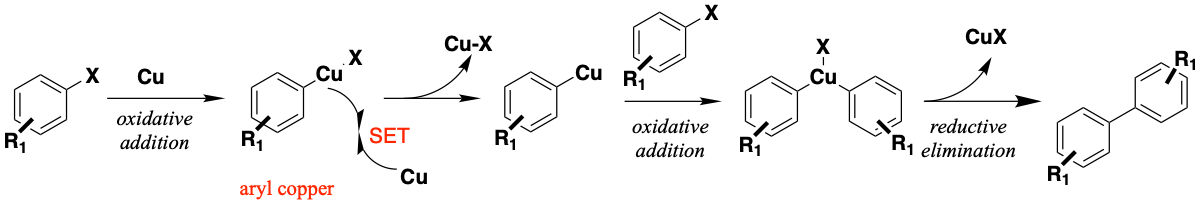
\includegraphics[width=1.0\columnwidth]{Fig/ullmann_mechanism.png}
%\caption{Mechanism of the Ullmann coupling reaction. SET stands for single-electron transfer.
%}
%\label{fig:classical}
%\end{figure}


%\textbf{Formation of organometallic intermediates on the Cu(111) surface.} Organic precursors are physisorbed on a metal surface before undergoing chemical transformations. Although the binding of chlorobenzene, bromobenzene and iodobenzene to Cu(111) calculated in this work is stronger than that obtained previously using the a different XC functional~\cite{jacs2013} the trends in the physisorption energies for different halogens are almost exactly the same (Table~\ref{table:bondlength}).

{\zhzh
\section{Disagreement between DFT simulation and experiment on Ullmann process}
In previous experimental study, dehalogenation requires a lower temperature than the C--C bond formation step~\cite{sur_sci01, sur_sci02, sur_sci03, ullmann_52, ullmann_68, ullmann_69, ullmann_88, ullmann_98}. However, DFT modeling reversely reported a higher barrier for the dissociation of halogen relative to the coupling step.
The reasons for this apparent mismatch between DFT modeling and experimental measurements are not yet clear and deserve a careful consideration in the future.

First, it is possible that the disagreement arises from the incorrect mechanistic interpretation of the measurements. For example, the dehalogenation may occur on surface defects (e.g. step edges, kinks, adatoms) which lower its activation barrier relative to the value calculated for the ideal surface~\cite{chemeurope2017}.

Second, it is possible the reasons for the mismatch are purely computational. One source of error might be the approximate nature of GGA functionals used in all previous works and in ours. While the accuracy of DFT can often be improved using hybrid XC functionals, it is computationally demanding to perform hybrid DFT for large periodic systems in this work. That is precisely why all previous computational studies of on-surface Ullmann coupling use GGA functionals and report the same mismatch between the dehalogenation and C—C bond formation steps~\cite{jacs2013, pccp2010}.

The most likely source of the improper ratio of the dehalogenation and the C—C bond formation barriers is the underestimation of the energy of covalent binding between the surface and organic groups by GGA functionals. This modeling error is not expected to alter key conclusions of our work because this study focuses entirely on the C—C bond formation step. The relative heights of the barriers of this step along the ideal and adatom pathways are expected to be less affected by the errors in the organic-surface binding.

}



\section{Formation of organometallic intermediates on Cu(111)} 

%\ifdefined\INTERNAL
%\subsection{Physisorption}
%\fi
%
%\ifdefined\INTERNAL
%\subsection{Dehalogenation}
%\fi

\begin{figure*}[bt]
\centering
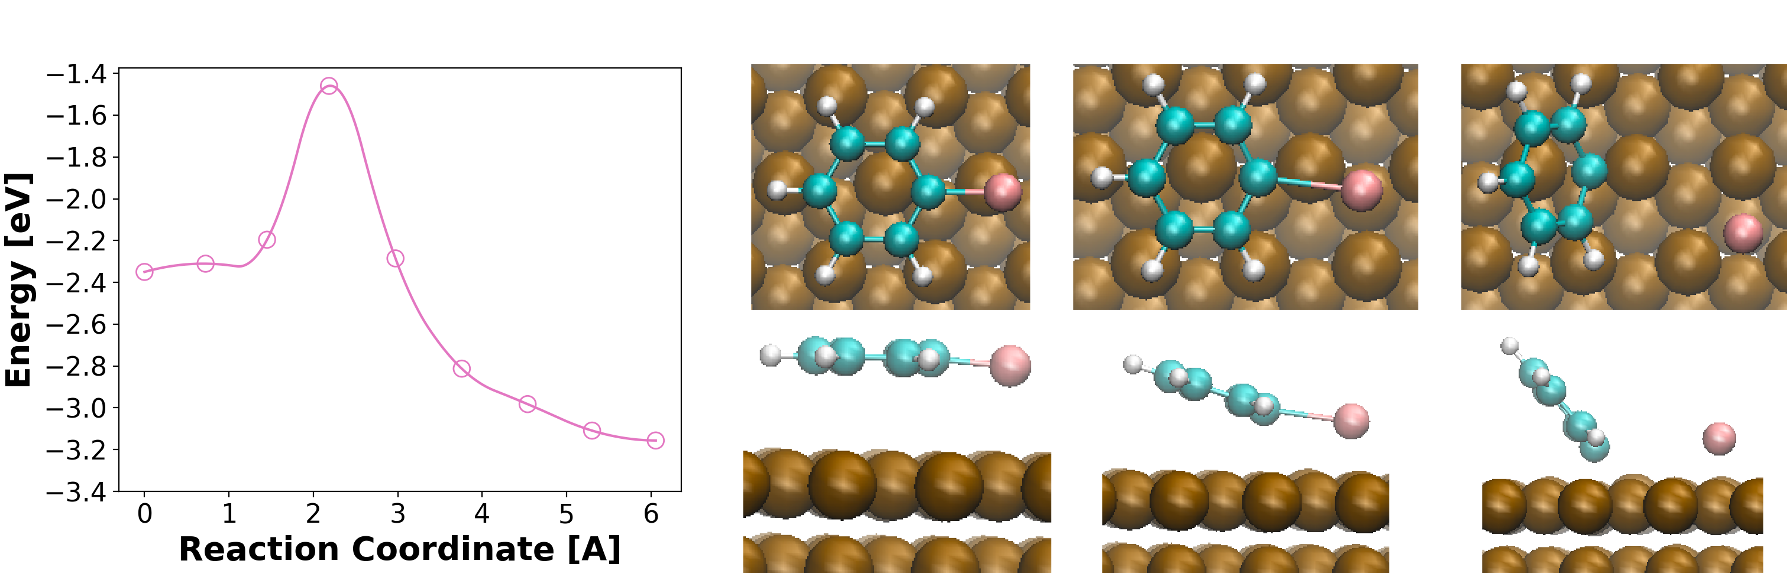
\includegraphics[width=1.0\textwidth]{Fig/dissociation_Br.pdf}
\caption{Dissociation of the C--Br bond on Cu(111). The energy diagram shows the NEB profile of the debromination process. In the structural images, orange, cyan, white, red spheres represent copper, carbon, hydrogen, bromine atoms, respectively.} %The dissociation of the C--Cl and C--I bonds is shown in \sinfo.
\label{fig:dissociation_Br}
\end{figure*}

\begin{figure*}[hbt]
\centering
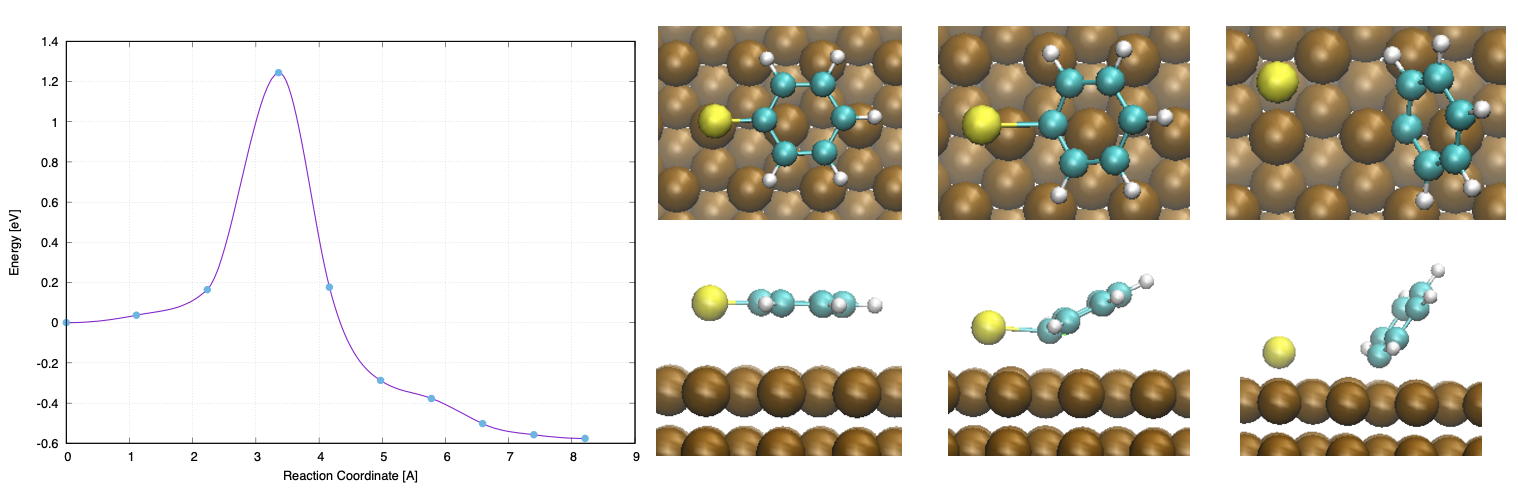
\includegraphics[width=1.0\textwidth]{Fig/dissociation_Cl.pdf}
\caption{Dissociation of the C--Cl bond on Cu(111). The energy diagram shows the NEB profile of the dechlorination process. In the structural images, orange, cyan, white, yellow spheres represent copper, carbon, hydrogen, chlorine atoms, respectively.}
\label{fig:dissociation_Cl}
\end{figure*}

\begin{figure*}[hbt]
\centering
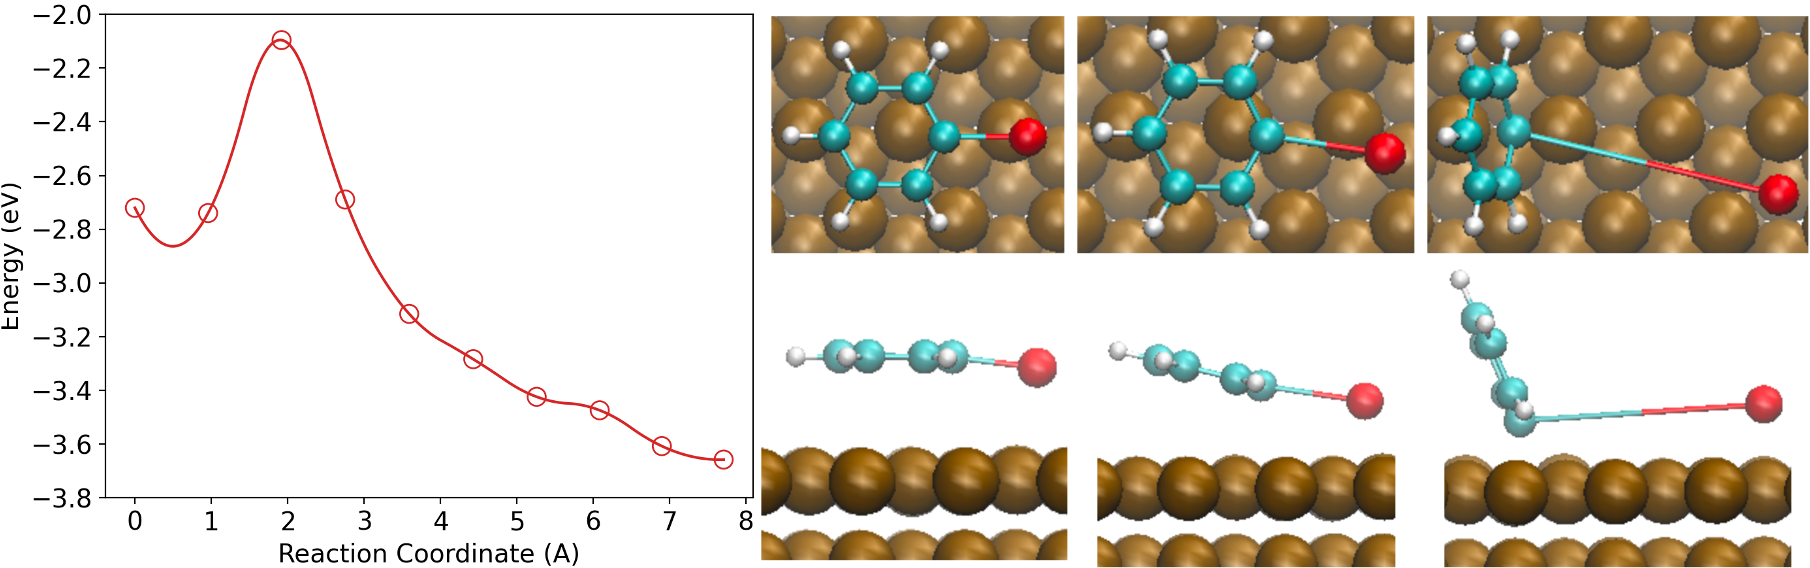
\includegraphics[width=1.0\textwidth]{Fig/dissociation_I.pdf}
\caption{Dissociation of the C--I bond on Cu(111). The energy diagram shows the NEB profile of the deiodination process. In the structural images, orange, cyan, white, purple spheres represent copper, carbon, hydrogen, iodine atoms, respectively.}
\label{fig:dissociation_I}
\end{figure*}

\begin{figure*}[hbt]
\centering
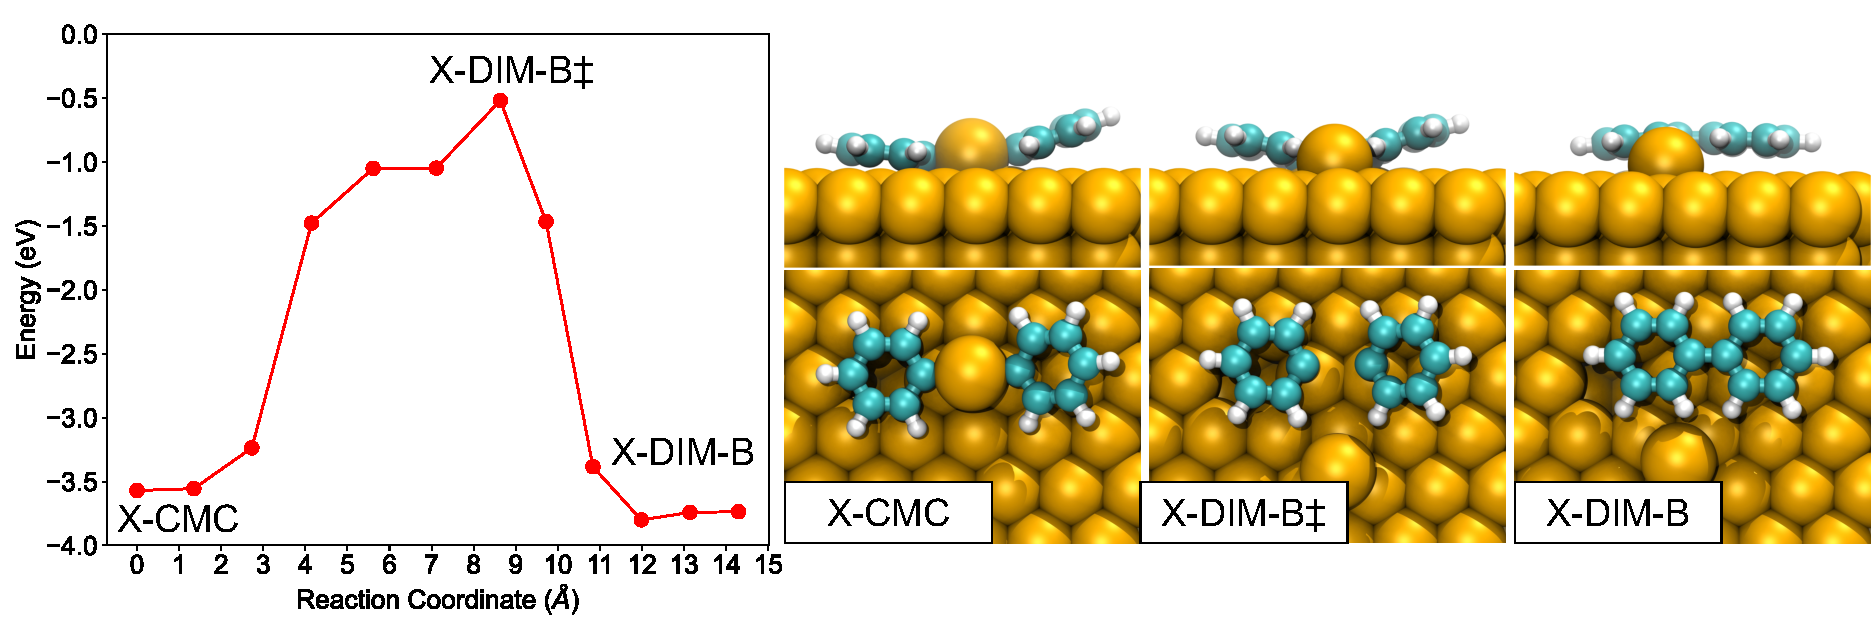
\includegraphics[width=1.0\textwidth]{Fig/AlterPath.pdf}
\caption{Alternative pathway for the adatom-catalyzed C--C formation on Cu(111). In this pathway, the formation of C--C bond and the separation of the adatom and biphenyl happen simultaneously rather than sequentially. In the structural images, orange, cyan, white, purple spheres represent copper, carbon, hydrogen, iodine atoms, respectively.}
\label{fig:AlterPath}
\end{figure*}

Organic precursors are physisorbed on a metal surface before undergoing chemical transformations. 
%REVIEW: Although the binding of chlorobenzene, bromobenzene and iodobenzene to Cu(111) calculated in this work (Fig.~\ref{fig:completeenergy}, \textbf{PHYS} state) is stronger than that obtained previously using the a different XC functional~\cite{jacs2013} the trends in the physisorption energies for different halogens are almost exactly the same (Table~\ref{SI-table:bondlength} in \sinfo).
%REVIEW: The strong binding between the surface and halogenated benzenes is primarily due to the interaction of (a) the $\pi$-system (b) halogen (choose one) and the surface. This follows from the analysis of the interaction energy between biphenyl and the metal (\SI{1.72}{\electronvolt}) and the van derWaals interaction of Br$_2$ molecule with the surface (\SI{1000}{\electronvolts}).
%
Fig.~\ref{fig:dissociation_Br} shows the structures of the initial, transition and final states for the debromination of the physisorbed bromobenzene on Cu(111). These states are labeled as \textbf{PHYS}, \textbf{DHAL$\ddagger$} and \textbf{DHAL}, respectively. Chlorobenzene and iodobenzene undergo similar structural transformation during the dehalogenation step (Figs.~\ref{fig:dissociation_Cl} and~\ref{fig:dissociation_I}).
%
%REVIEW (Numbers should be verified): Unlike analogous reactions in the solution, dehalogenation reactions on the copper surface are all exothermic. DFT results have demonstrated that the energy barrier of nucleophilic substitution of chlorobenzene and bromobenzene in solution are \SI{1.11}{\electronvolt} and \SI{1.18}{\electronvolt}~\cite{ullmann_86}.
%
The amount of energy released in the dehalogenation step on Cu(111) surface increases from chlorobenzene (\SI{0.58}{\electronvolt}) to bromobenzene (\SI{0.81}{\electronvolt}) and to iodobenzene (\SI{0.96}{\electronvolt}) (Fig.~\ref{main-fig:completeenergy} and Table~\ref{table:bondlength}).
The energy barriers follow the opposite trend decreasing from chlorobenzene (\SI{1.24}{\electronvolt}) to bromobenzene (\SI{0.89}{\electronvolt}) and to iodobenzene (\SI{0.63}{\electronvolt}), in agreement with the Bell-Evans-Polanyi principle.
The calculated energies are in qualitative agreement with the trend in experimentally measured dehalogenation temperatures (Table~\ref{table:experimental-temperatures})~\cite{ullmann_52,ullmann_87,ullmann_67} and with the previous calculations on this~\cite{jacs2013} and similar systems.
%{\comm REVIEW only becuase the trend is reproduced only roughly. On Cu(111), iodobenzene has been observed to dissociate at \SI{175}{\kelvin}~\cite{ullmann_87} while bromobenzene dissociates at \SI{160}{\kelvin}~\cite{ullmann_67}. There is no data the dehalogenation temperature of chlorobenzene, but it can be inferred from the existing data on dihalogenated precursors (Table~\ref{table:exp-temp}) that chlorobenzene dissociates at significantly higher temperature than both bromobenzene and iodobenzene.}

%REVIEW: It should be noted that the dehalogenation of bromobenzene and iodobenzene on Cu(111) has been investigated previously~\cite{jacs2013} using optB86b exchange-correlation functional and smaller slab size, the molecular orientation on Cu(111) is identical with our model. The previous energy barrirer of this step are \SI{0.66}{\electronvolt} (bromobenzene), \SI{0.44}{\electronvolt} (iodobenzene). The previous energy change is \SI{-0.68}{\electronvolt} (bromobenzene) and \SI{-0.81}{\electronvolt} (iodobenzene). The slight difference in the energy value can be interpreted by different functional usage and our larger slab model for computation.

%REVIEW: The following paragraph discusses details that are not relevant to the current topic. It is commented out and can be restored when REVIEW is written.
%{\zhzh
%Selected geometric parameters of the intermediates have also been summarized in Table~\ref{table:bondlength}. 
%In \textbf{PHYS} of halobenzene, the distance between carbon and halogen is consistent with the C--halogen covalent bond length (\SI{1.76}{\angstrom} in chlorobenzene, \SI{1.91}{\angstrom} in bromobenzene and \SI{2.14}{\angstrom} in iodobenzene, respectively) in gas phase calculated based on B3LYP functional. These distances show a continued growth till \textbf{DHAL} states, and dissociated halogen atoms all occupy the hollow sites on Cu(111) surface in the end of dehalogenation. Interestingly, C--halogen distances in three different \textbf{DHAL$\ddagger$} show consistent approximately \SI{0.5}{\angstrom} longer than corresponding C--halogen lengths in \textbf{PHYS} , suggesting that different dehalogenation reactions on Cu(111) follow similar mechanisms.
%The angle of phenyl ring also suffers successively changes, parallel in \textbf{PHYS}, tilt in the process of dehalogenation and finalize with an apparent slope in \textbf{DHAL}. The interaction between unsaturated carbon and copper atom shortens their distance to same \SI{2.01}{\angstrom} in three different \textbf{DHAL} states, and these copper atoms are all raised approximately by \SI{0.12}{\angstrom} from their original positions.
%The same C--Cu distances in \textbf{DHAL} suggest that the dissociated halogen atoms have little effect on phenyl--Cu intermeidate. However, halogen atoms have obvious influence on dissociated phenyl ring, resulting in their different tilt angles, deiodinated phenyl ring is inclined around \SI{70}{\degree} to metal surface, larger than debrominated and dechlorinated phenyl rings both at around \SI{50}{\degree}.
%}

%\ifdefined\INTERAL
%\subsection{Formation of carbon-metal-carbon intermediates}
%\fi

The formation of carbon-metal-carbon organometallic intermediates (\textbf{CMC}) from two phenyl radicals (\textbf{DHAL-2}) is slightly endothermic with the energy ranging from \SIrange{0.17}{0.25}{\electronvolt} (Fig.~\ref{main-fig:completeenergy} and Table~\ref{table:bondlength}). Experimentally, the dehalogenation and formation of the bridge structure occur at the same temperature indicating that the two phenyl groups need to overcome only a small energy barrier to approach each other~\cite{ullmann_88}. 
%REVIEW: Gold surface is an exception that C--Au--C intermediates are rarely observed in experiment due to fast proceeding to coupling product after dehalogenation~\cite{ullmann_93, ullmann_100, ullmann_101, ullmann_102, ullmann_103, jacs2011}.
%
The two phenyl groups in the \textbf{CMC} state lift their common copper atom \SI{0.53}{\angstrom} above its ideal-surface position, which noticeably higher than the \SI{0.12}{\angstrom} raise in the \textbf{DHAL-2} state (Table~\ref{table:bondlength}).

%\textbf{DHAL-2} used here is well matched to the experimental STM image shown in Fig.~\ref{fig:organ}, the dissociated bromine atoms sit around in the formation of phenyl--Cu--phenyl structures. 
%The distance between two carbon atoms in the C--Cu--C bridge is \SI{3.10}{\angstrom}, which is \SI{1.61}{\angstrom} longer than the length of the connecting C--C in biphenyl. The angle of two phenyl rings connected to the Cu atom with respect to the surface are both \SI{52}{\degree}, this angle is the same as the tilt of a single phenyl in DHAL (\SI{52}{\degree}).

%REVIEW: This step was reported to be exothermic in the previous work~\cite{pccp2010}. Two dehalogenated phenyl radicals are infinitely far this time, while they interact with adjacent copper atoms in the previous work. %I think this is a clumsy explanation. The repulsion between phenyl radicals results in a higher energy initial configuration and lead to such inconsistency.

%Formation of C--Cu--C bridge intermediate has been proven to play a significant role in the creation of adatom in the surface Ullmann coupling. The interaction is potentially sufficient to extract an ideal surface copper atom out.


\begin{table*}
\centering
\caption{Structural and energetic characteristics of the intermediates in the dehalogenation step on Cu(111). The energies are relative to \textbf{SURF}.}
\label{table:bondlength}
\begin{tabular}{ llccccc  }
 \hline
 \hline
  & & & & Barrier & & Change \\
  & Hal. & \textbf{PHYS}$^{a}$ & \textbf{DHAL$\ddagger$}$^{b}$ & $\Delta^{(b-a)}$ & \textbf{DHAL}$^{c}$ & $\Delta^{(c-a)}$ \\ 
 \hline 
 \multirow{3}{*}{C--Hal (\si{\angstrom})} & Cl & 1.74 & 2.18 & +0.44 & 3.99 & +2.25 \\ 
 %\cline{2-5}
 & Br & 1.91 & 2.46 & +0.55 & 4.10 &+2.19 \\ 
 %\cline{2-5}
 & I & 2.12 & 2.61 & +0.49 & 5.10 &+2.98 \\ 
 %\cline{2-5}
 \hline
 \multirow{3}{*}{C--Cu (\si{\angstrom}) } & Cl & 3.54 & 2.52 & -1.02 & 2.01 & -1.53 \\ 
 & Br & 3.40 & 2.77 & -0.63 & 2.01 & -1.39 \\ 
 & I &3.42 & 2.73 &-0.69 & 2.01 & -1.41 \\ 
 \hline
 \multirow{3}{*}{Hal--Cu (\si{\angstrom}) } & Cl & 2.99 & 2.37 & -0.62 & 3.50 & +0.51 \\ 
 & Br & 2.89 & 2.50 & -0.49 & 3.57 & +0.68 \\ 
 & I &2.80 & 2.64 &-0.16 & 3.74 & +0.94 \\ 
 \hline
 \multirow{3}{*}{E (\si{\electronvolt}) } & Cl & -1.07 & 0.17 & 1.24 &-1.65 & -0.58 \\ 
 & Br &-1.14 &-0.25 & 0.89 & -1.95& -0.81 \\ 
 & I  & -1.32 & -0.69 & 0.63 & -2.28& -0.96 \\ 
 \hline
 \multirow{2}{*}{E (\si{\electronvolt})~\cite{jacs2013}} & Br &-0.95 & & 0.66 & & -0.68 \\ 
 & I & -1.12 & & 0.40 & & -0.81 \\ 
 \hline
 \hline
\end{tabular}
\end{table*}


\begin{table*}
\centering\caption{Minimum experimentally measured temperatures (\si{\kelvin}) necessary for the completion of two Ullmann coupling steps.}
\begin{tabular}{ lcccccc }
 \hline
 \hline
  & \multicolumn{3}{c}{Dehalogenation} & \multicolumn{3}{c}{C--C bond formation} \\
  &\multicolumn{1}{c}{Cu} &\multicolumn{1}{c}{Ag} & \multicolumn{1}{c}{Au} & \multicolumn{1}{c}{Cu} &\multicolumn{1}{c}{Ag} &\multicolumn{1}{c}{Au}\\
 \hline
 Iodobenzene             &175\cite{sur_sci01} &200\cite{sur_sci02} &200-250\cite{sur_sci03} &350\cite{ullmann_68} &300-370\cite{ullmann_68} &250\cite{sur_sci03}\\
 Bromobenzene  &160\cite{ullmann_67} &$\leq$ 197\cite{sur_sci02}  &  &350\cite{ullmann_67}  &$\leq$ 350\cite{sur_sci02}  & \\
 Dichlorobenzene &420\cite{ullmann_52} & & &470\cite{ullmann_52} & & \\
 Dibromobenzene &$\leq$ 300\cite{ullmann_52} & & &470\cite{ullmann_98}  & & \\
 Diiodobenzene &$\leq$ 300\cite{ullmann_52} & & &500 \cite{ullmann_88} & & \\
 \hline
 \hline
\end{tabular}
\label{table:experimental-temperatures}
\end{table*}

\begin{table*}
\centering
\caption{Characterization of the intermediates in the ideal-surface pathway. %The states are labeled as in Fig.~\ref{fig:completeenergy}. 
The energies are relative to \textbf{SURF}.
%For the coupling step, the energy change and barrier for different halobenzenes are exactly same due to the absence of halogen atoms in this step.
}
\label{table:idealsurface}
\begin{tabular}{ llcccccccc  }
 \hline
 \hline
  & & &  & Barrier & & Change & &\\
  & Met./Hal. & \textbf{CMC}$^{a}$ & \textbf{DIM$\ddagger$}$^{b}$ & $\Delta^{(b-a)}$ &  \textbf{DIM}$^{c}$ & $\Delta^{(c-a)}$  & \textbf{DSRB} & \textbf{PROD} \\ 
 \hline 
 C--C (\si{\angstrom}) & Cu/Any & 3.10 & 2.28 & -0.82 & 1.49 & -1.61 & 1.49 & 1.49 \\ 
 \hline
 C--Cu (\si{\angstrom}) & Cu/Any & 2.06 & 2.03 & -0.03 & 3.22 & +1.16 & & \\
 \hline
 Cu lift (\si{\angstrom}) & Cu/Any & 0.53 & 0.49& -0.04  & 0.00 & -0.53 & 0.00 & 0.00 \\
 \hline
 \multirow{3}{*}{E (\si{\electronvolt}) } & Cu/Cl & -3.05 &-2.56 &+0.49 & -5.05 & -2.00& -3.33&0.85\\ 
 & Cu/Br & -3.73 & -3.24 &+0.49 & -5.73 & -2.00& -4.01&0.07\\ 
 & Cu/I  & -4.38 & -3.89 & +0.49 & -6.38 & -2.00& -4.66&-0.71\\ 
 \hline
 & Ag/Br & -2.01 & -1.39 & +0.62& -4.78 &-2.77 &-3.43 & 0.07\\ 
 \hline
 & Au/Br & -0.88 & -0.74 & +0.14& -3.59 &-2.71 &-2.03 & 0.07\\ 
 \hline
 E (\si{\electronvolt})~\cite{pccp2010} & Cu/Any &  &  & +0.38& & -1.90 & & \\
 \hline
 E (\si{\electronvolt})~\cite{jacs2013} & Cu/Any & &  & +0.14& & -2.06 & &\\
 \hline
 \hline
\end{tabular}
\end{table*}


\begin{table*}
\centering
\caption{Characterization of the intermediates in the $[11\bar{2}]$ adatom pathway. The energies are relative to \textbf{SURF}. 
}
\label{table:adatom-longitude}
\begin{tabular}{ llcccccccccccc  }
 \hline
 \hline
  & & & & Barrier & & Change & & Barrier & &Change&\\
  & M./Hal. & \textbf{CMC}$^{a}$ & \textbf{X-CMC$\ddagger$}$^{b}$ & $\Delta^{(b-a)}$ & \textbf{X-CMC}$^{c}$ &$\Delta^{(c-a)}$ & \textbf{X-DIM$\ddagger$}$^{d}$ & $\Delta^{(d-c)}$ & \textbf{X-DIM-A}$^{e}$ &$\Delta^{(e-c)}$ & \textbf{X-DIM-B}  \\ 
 \hline
 \hline 
 {C--C (\si{\angstrom})} & Cu/Any & {3.10} & {3.53} & {+0.43} & {3.86} &{+0.76} & {2.56} & {-1.30} & {1.51} &{-2.35} &{1.50}\\ 
 \hline
 {C--M (\si{\angstrom}) } & Cu/Any & {2.06} & {1.85} & {-0.21} & {1.94} &{-0.12} & {1.89} & {-0.05} & {2.16} &{+0.22} & \\ 
 \hline
 {M lift (\si{\angstrom}) } & Cu/Any & {0.53} & {1.58} & {+1.05} & {1.97} &{+1.44} & {1.81} & {-0.16} & {1.71} &{-0.26} & \\ 
% \hline
% \hline
 \hline
 \multirow{3}{*}{E (\si{\electronvolt}) } & Cu/Cl & -3.05 &-2.34 & +0.71 &-2.89 &+0.16 &-1.11 & +1.78 & -3.37&-0.48&-3.29\\ 
 & Cu/Br &-3.73 &-3.02 &+0.71 & -3.57 &+0.16 &-1.79 & +1.78 & -4.06 & -0.48&-3.97 \\ 
 & Cu/I  & -4.38 & -3.67 & +0.71 & -4.22 &+0.16 &-2.44 & +1.78 & -4.70 & -0.48&-4.62\\ 
 \hline
 E (\si{\electronvolt}) & Ag/Br &-2.01 &-1.58 &+0.43 &-1.87 &+0.14 &-0.35 &+1.52 &-3.13 &-1.26 &-3.48 \\ 
 E (\si{\electronvolt}) & Au/Br &-0.88 &-0.52 &+0.36 &-0.52 &+0.36 &-0.32 &+0.20 &-2.17 &-1.65 &-2.04 \\
  \hline
 \hline
\end{tabular}
\end{table*}

\begin{table*}
\centering
\caption{Characterization of the intermediates in the $[1\bar{1}0]$ adatom pathway on Cu(111). Energies are reported relative to the \textbf{SURF} state.}
\label{table:adatom-110}
\begin{tabular}{ lccccccccccccc  }
 \hline
 \hline
 & & & & Barrier & & Change & & Barrier & &Change&\\
 & Met./Hal. & \textbf{CMC}$^{a}$ & \textbf{X-CMC$\ddagger$}$^{b}$ & $\Delta^{(b-a)}$ & \textbf{X-CMC}$^{c}$ &$\Delta^{(c-a)}$ & \textbf{X-DIM$\ddagger$}$^{d}$ & $\Delta^{(d-c)}$ & \textbf{X-DIM-A}$^{e}$ &$\Delta^{(e-c)}$ & \textbf{X-DIM-B}  \\ 
 \hline 
 {C--C (\si{\angstrom})} & Cu/Any & {3.10} & {3.55} & {+0.45} & {3.89} &{+0.79} & {2.53} &{-1.36} & {1.50} &{-2.39}\\ 
 \hline
 {C--Cu (\si{\angstrom}) } & Cu/Any & {2.06} & {1.85} & {-0.21} & {1.96} &{-0.10} & {1.90} &{-0.06} & {2.14} &{+0.18} &{} \\ 
 \hline
 {Cu$_{\rm lift}$ (\si{\angstrom}) } & Cu/Any & {0.53} & {1.68} & {+1.16} & {2.02} &{+1.49} & {1.77} & {-0.25} & {1.76} &{-0.26} &{0.00}\\ 
 \hline
 \multirow{3}{*}{E (\si{\electronvolt}) } & Cu/Cl & -3.05 &-1.67 & +1.38 &-3.26 &-0.21 & -1.25 & +2.01& -3.42&-0.16&-3.29 \\ 
 & Cu/Br &-3.73 &-2.35 &+1.38 & -3.94 &-0.21 & -1.93 & +2.01 & -4.11 & -0.16&-3.97 \\ 
 & Cu/I  & -4.38 & -3.00 & +1.38 & -4.59 &-0.21 & -2.58& +2.01 & -4.76 & -0.16&-4.62\\ 
 \hline
 \hline
\end{tabular}
\end{table*}


%\begin{figure*}[h!]
%\centering the process of
%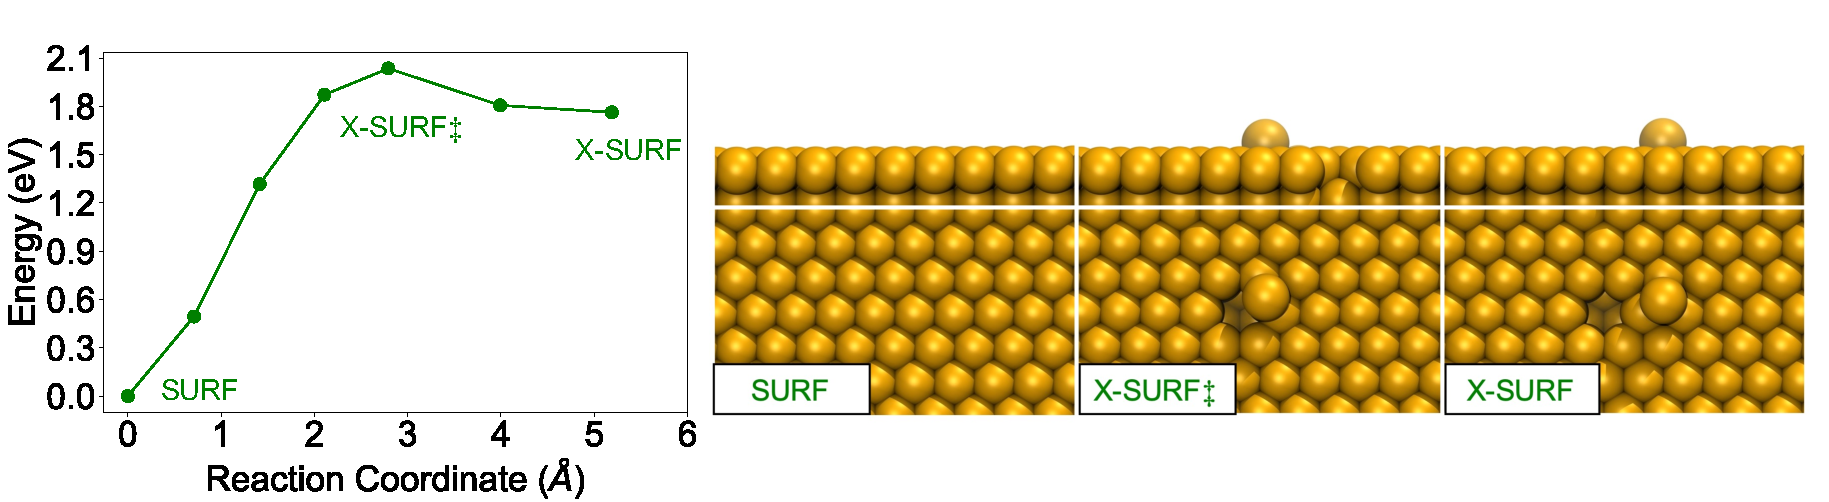
\includegraphics[width=1.0\textwidth]{Fig/pureadatomform.pdf}
%\caption{Energetics of an adatom formation on the clean Cu(111) surface.}
%\label{fig:cleanatomform}
%\end{figure*}

%\begin{figure}[hbt]
%\centering
%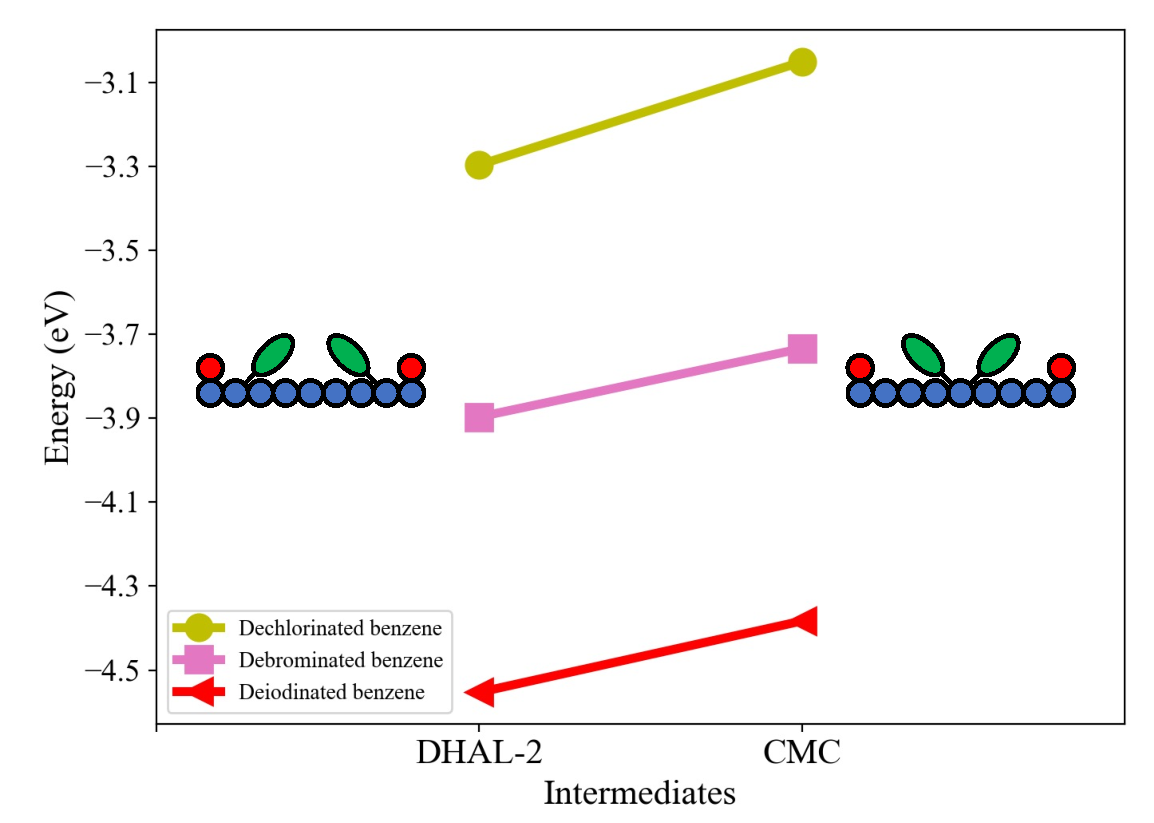
\includegraphics[width=0.45\textwidth]{Fig/FormingC-Cu-C.pdf}
%\caption{
%Energy diagram of forming C--Cu--C bridge intermediates structures from dechlorinated, debrominated and deiodinated benzene. The energy is computed as the difference between 2 $\times$ dehalogenated intermediates (left geometry) and C--Cu--C bridge intermediate structure $+$ two bromine atoms on Cu(111) surface. The blue circles represent chlorine, bromine or iodine atoms respectively in three situations. Yellow line with circle points is dechlorinated benzene to C--Cu--C, pink line with square points is debrominated benzene to C--Cu--C and red line with triangle points is deiodinated benzene to C--Cu--C.}
%\label{fig:formingBridge}
%\end{figure}

\section{Comparison of the dehalogenation and C--C bond formation energy barriers}

It should be noted that the calculated energy barriers for the dehalogenation of bromobenzene on Cu(111), Ag(111) and Au(111) surfaces (0.89, 1.20, \SI{1.46}{\electronvolt}, respectively) are higher than the energy barriers for the C--C bond formation step (0.49, 0.62, \SI{0.14}{\electronvolt}, respectively). This results are inconsistent with the temperatures required for the completion of these two Ullmann coupling steps in experiments. Table~\ref{table:experimental-temperatures} indicates that on Cu and Ag surfaces additional heating is necessary to complete the C--C bond formation step, which means that the C--C bond formation barrier should be higher than the dehalogenation barrier on these surfaces. Thus, it appears that the calculated barriers for the dehalogenation step are too high compared to those for the C--C bond formation step.

The reasons for this apparent mismatch between DFT modeling and experimentally measurements are not clear. It is possible that the disagreement arises from the incorrect mechanistic interpretation of the measurements. For example, the dehalogenation may occur on surface defects (e.g. step edges, kinks, adatoms), which are expected to lower the activation barrier of the dehalogenation compared to that on the ideal surface~\cite{chemeurope2017}. It is possible the reasons for the mismatch are purely computational. One source of error might be the approximate GGA exchange-correlation (XC) functionals used in this and all previous works~\cite{RZK-references}. In this case, the underestimation of the energy of covalent binding between the surface and organic groups by GGA functionals can be responsible for the incorrect relative barrier heights. This modeling error is not expected to alter key conclusions of the work because this study focuses entirely on the  C--C bond formation step. The relative heights of the barriers of this step along the ideal and adatom pathways are expected to be less affected by the errors in the organic-surface binding.

\section{Conditions for competitive adatom catalysis}

%The analysis of the three metals performed in this work raises a tantalizing question whether it is possible to find a metal surface capable of catalyzing the coupling of two phenyl groups through an efficient and competitive adatom pathway. 

The data collected in this work shows that the strengthening of the phenyl-adatom binding relative to the phenyl-surface binding -- further denoted as $X$ -- is important for two reasons. First, $X$ determines the energetics of the C--C bond formation step. For example, there is a nearly linear relation between $X$ and $\Delta B$ -- the difference in the C--C bond formation activation barriers in the adatom and ideal-surface pathways (Figure~\ref{main-fig:onlysurface}b):
% 
\begin{equation} \label{eq:relation1}
\Delta B = 0.898 X
\end{equation}
%
Second, $X$ determines the energetics of the extraction step as well. As described in the main text, the energy required for the unassisted adatom extraction -- further denoted as $Y$ -- is compensated by $X$ when phenyl groups are bonded to the extracted adatom. It is reasonable to assume that metals with lower $Y$ (but same $X$) will have lower energy of phenyl-assisted extraction. For (hypothetical) metals with sufficiently low $Y$, the energy cost of the adatom extraction will be fully compensated by $X$, resulting in the phenyl-assisted extraction that is thermoneutral. 

To predict the energy of the phenyl-assisted extraction $E_{AX}$ (i.e. $AX$ stands for assisted extraction) for a metal with known numerical values of $X$ and $Y$, the value of $Y$ can be corrected by some (yet unspecified) amount $\text{TNE}$, which will be different for different $X$
%
\begin{equation} \label{eq:relation2}
\begin{split}
E_{AX} = Y - \text{TNE}(X)
\end{split}
\end{equation}
%
$\text{TNE}$ here stands for ThermoNeutral Extraction because this is the physical meaning of this correction: if $Y$ happens to be equal to $\text{TNE}$ then the phenyl-assisted extraction will be thermoneutral.

The collected DFT data can be used to determine $\text{TNE}$ as a function of $X$ (note that this function will be different if other organic precursors are of interest). Indeed, the values of $X$, $Y$ and $E_{AX}$ are known for three metals surfaces and the phenyl group. This allows to compute values of $\text{TNE}$ at three points $X$ and inter- or extrapolate for other values of $X$ using a convenient fitting function. Remarkably, the three datapoints lie on a straight line (Fig.~\ref{main-fig:conclusion}), giving the following almost perfect fit for $\text{TNE}(X)$
%
\begin{equation} \label{eq:TNEfit}
\begin{split}
\text{TNE}(X) = 1.026 + 0.420 X
\end{split}
\end{equation}
%
where the constant term is in \si{\electronvolt} and the coefficient in the linear term is dimensionless. 

%The line of thermoneutral extraction (TNE) is a shows what Y should a hypothetical metal with X have to exhibit the thermoneutral phenyl-assisted adatom extraction. Points lying below this line are characterized by exothermic assisted extraction and above this line by endothermic extraction. The vertical distance between a point $(X,Y)$ and the line is equal to the absolute energy of the phenyl-assisted adatom extraction:
%%
%\begin{equation} \label{eq:relation2}
%\begin{split}
%E_{\text{AEX}} = Y - \text{TNE}(X)
%\end{split}
%\end{equation}
%%

%The line of TNE is calculated by fitting a straight line to several points of TNE. Point of TNE is a point in the X-Y space at which the phenyl-assisted adatom extraction from the surface of a hypothetical metal is expected to have precisely zero energy.  The Y-position of a point of TNE is calculated from the DFT data for the metal by subtracting the energy of the phenyl-assisted adatom extraction from the clean-surface adatom extraction energy. The X-position of the point of TNE is assumed to be the same as the X-position of the metal described by DFT.

The established relations are required to determined the condition for the competitive adatom catalysis for the coupling of two phenyl groups 
%
\begin{equation} \label{eq:compete}
\begin{split}
\frac{r^{\text{adatom}} }{ r^{\text{ideal}} } &> 1
\end{split}
\end{equation}
%
where the rates of the product formation on the ideal surface and adatom are compared. The expressions for the rate on the ideal surface can be written as
%
\begin{equation}
\begin{split}
r^{\text{ideal}} &= \frac{d[\text{DIM}]}{dt} = k^{\text{DIM}\ddagger} [\text{CMC}]   \\
&= A \exp\left[ -\frac{B_0}{k_B T} \right] [\text{CMC}] 
\end{split}
\end{equation}
%
where $A$ is the Arrhenius prefactor and $B_0$ is the C--C bond formation energy
%
\begin{equation}
\begin{split}
B_0 = E(\text{DIM}\ddagger) - E(\text{CMC}) 
\end{split}
\end{equation}
%
It should be noted that the free energies, required to determine the rate and equilibrium constants are substituted by electronic energies, which can be obtained from DFT readily.

The rate of the product formation along the ideal path can be obtained assuming that the adatom extraction step is fast
%
\begin{equation}
\begin{split}
r^{\text{adatom}} &= \frac{d[\text{X-DIM-A}]}{dt} = k^{\text{X-DIM}\ddagger} K_{AX} [\text{CMC}] 
\end{split}
\end{equation}
%
where
%
\begin{equation}
\begin{split}
k^{\text{X-DIM}\ddagger} &= A' \exp\left[ -\frac{B_0+\Delta B}{k_B T} \right] \\
K_{AX} &= \exp\left[ -\frac{E_{AX}}{k_B T} \right] 
\end{split}
\end{equation}
%
Therefore, the expression for the rate along the adatom pathway is 
%
\begin{equation}
\begin{split}
r^{\text{adatom}} &= A' \exp\left[ -\frac{E_{AX} +B_0+\Delta B}{k_B T} \right] [\text{CMC}] 
\end{split}
\end{equation}
%

If it is assumed that $A=A'$ and the rate expressions are plugged into the condition for the competitive adatom catalysis, Eq.~\ref{eq:compete}, it reduces to
%
\begin{equation}
\begin{split}
E_{AX} + \Delta B &< 0
\end{split}
\end{equation}
%
To interpret this condition for the competitive adatom catalysis: the assisted extraction should be sufficiently exothermic ($E_{AX} < 0$) to outweigh the always slower C--C bond formation on adatoms $\Delta B > 0$.

Fortunately, both $E_{AE}$ and $\Delta B$ can be obtained from the DFT data as shown in Eqs.~(\ref{eq:relation1}), (\ref{eq:relation2}) and~(\ref{eq:TNEfit}), giving the following condition for the competitive adatom catalysis for the coupling of two phenyl groups: ~\cite{book-test1}
%
\begin{equation}
\begin{split}
Y &< 1.026 - 0.478 X
\end{split}
\end{equation}
%
This inequality defines the region shown in Fig.~\ref{main-fig:conclusion} in the main text.


{\zhzh \section{Entropy correction with mobile models}
In statistical thermodynamics, the partition sum $Q_{\text{sys}}$ of the system consisting of N molecules can be computed as: %
\begin{equation}
\begin{split}
Q_{\text{sys}} = \frac{1}{N!} q^{N}_{\text{mol}} 
\end{split}
\end{equation}
%
and the partition function of each molecule contains four components: translational, rotational, vibrational and electronic terms (ignore nuclear partition function)
%
\begin{equation}
\begin{split}
q_{\text{mol}} = q_{\text{elec}q_{\text{rot}}q_{\text{vib}}}q_{\text{tran}}
\end{split}
\end{equation}
%
And the Helmholtz free energy per molecule in the system can be derived by: 
%
\begin{equation}
\begin{split}
A = - \frac{k_BT}{N}lnQ
\end{split}
\end{equation}
%

The molecules of all reaction states are divided into two categories: in gas phase or on surface. For the molecules in gas phase, electronic, translational and vibrational terms were considered since vibration motion makes less contribution to the free energy in this modeling system:

\begin{equation}
\begin{split}
% q_{\text{tran}} &= \left(\frac{2\pi mk_BT}{h^2}\right)^{\frac{3}{2}} V = \frac{k_BT}{P}\left(\frac{2\pi Mk_BT}{h^2}\right)^\frac{3}{2} \\
% q_{\text{rot}} &= \frac{\sqrt{\pi}}{\sigma} \left(\frac{8\pi^2k_BT}{h^2}\right)^\frac{2}{3} \\
% q_{\text{ele}} &= w_{GS}\text{exp}\left(-\frac{E_{GS}}{k_BT}\right)
A &= -\frac{k_BT}{N}ln(q_{\text{elec}}q_{\text{rot}}q_{\text{tran}}) \\
&=  E_{GS} - k_BT\log{w_{GS}} \\
&\quad - k_BT\log{\left[\frac{\sqrt{\pi}}{\sigma} \left(\frac{8\pi^2k_BT}{h^2} \right)^{\frac{2}{3}}(I_aI_bI_c)^{\frac{1}{2}} \right]} \\
&\quad -k_BT\log{\left[ \left( \frac{P}{k_BT} \right) \left( \frac{2\pi Mk_BT}{h^2}\right)^{-\frac{3}{2}}  \right]}
\end{split}
\end{equation}
Where the $E_{GS}$ and $w_{GS}$ is the electronic energy of ground state and its degeneracy, $\sigma$ is the symmetry number of molecule, $I$ is the moments of inertia, P and T are the pressure and temperature of the system, M is the mass of free mobile molecule.

For the intermediates adsorbed on surface, the vibration and rotation vanish since surface defines their motion into 2D mode. The translational partition function can adopt a 2D forms~\cite{ullmann_172}:
\begin{equation}
\begin{split}
A &= -\frac{k_BT}{N}ln(q_{\text{elec}}q_{\text{tran}}) \\
&=  E_{GS} - k_BTln\log{w_{GS}} \\
&\quad -k_BT\log{\left[ \rho \left( \frac{2\pi Mk_BT}{h^2}\right)^{-1}  \right]}
\end{split}
\end{equation}
Where $\rho$ is the concentration of molecule on surface.


}

\begin{figure*}[bt]
\centering
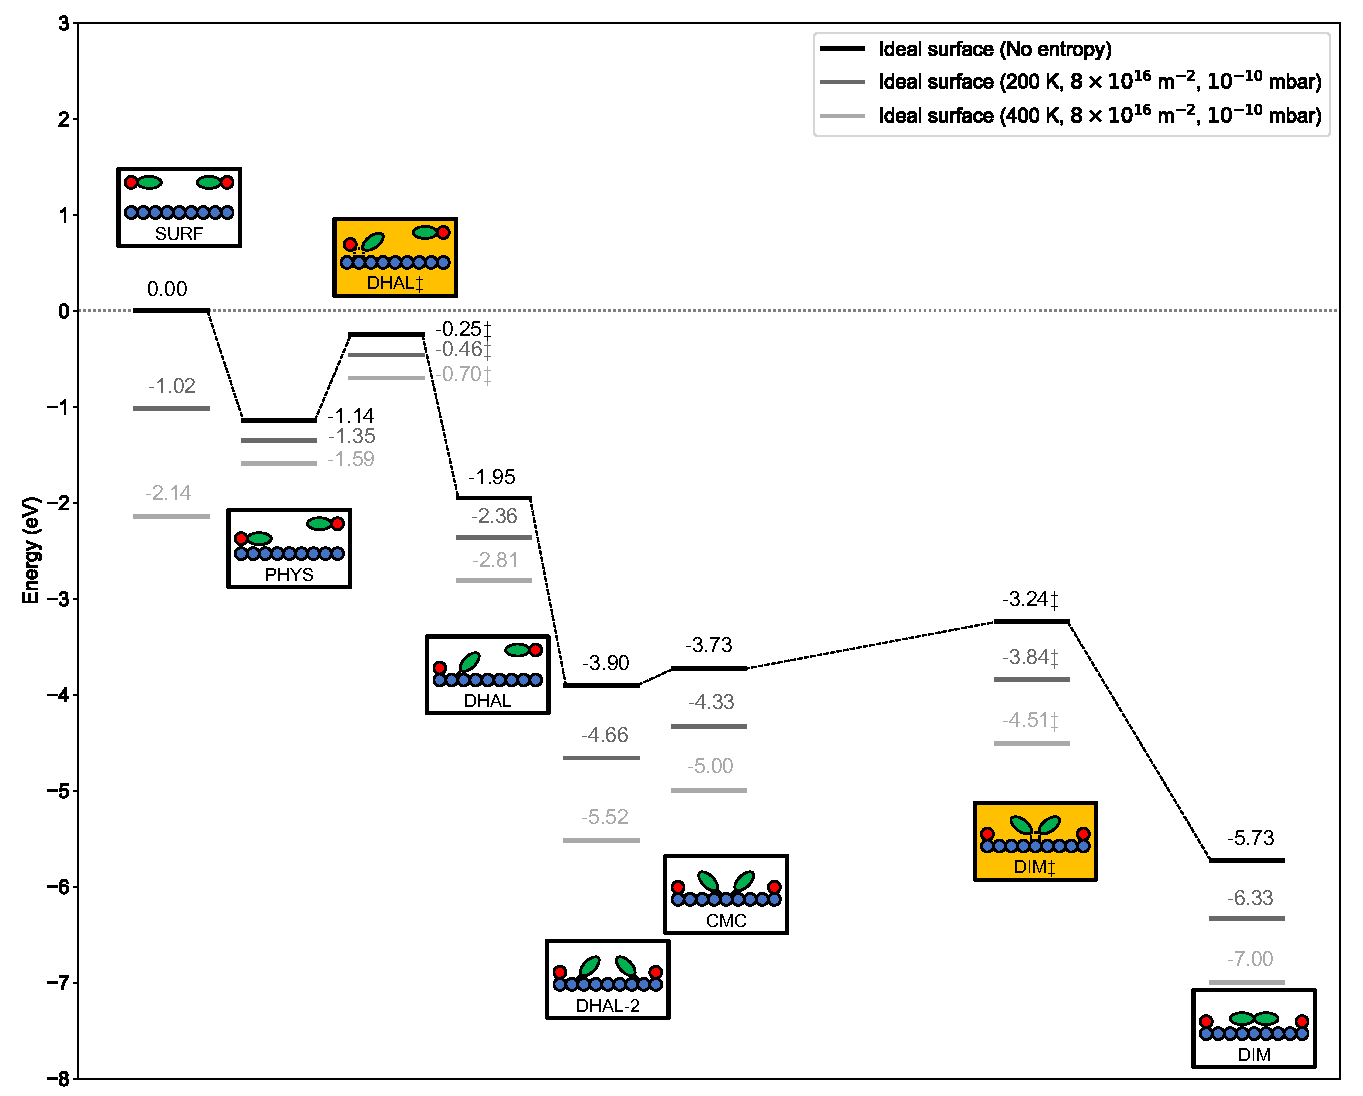
\includegraphics[width=0.96\textwidth]{Fig/Entropy_ideal.pdf}
\caption{Energy profile of the Ullmann reaction of bromobenzene on Cu(111) after applying entropy effects following ideal surface pathway. Levels shown with black color are states without additional entropy-related functions, whereas the dimgrey states are with a entropy correction at \SI{200}{\kelvin} temperature and grey states are at \SI{400}{\kelvin} temperature. Both entropy correction are completed at \SI{e-10}{\milli\bar} UHV condition. The concentration of molecule is approximately 0.8 molecule per \si{\nano\metre\squared}}.
\label{fig:entropy_ideal}
\end{figure*}

\begin{figure*}[bt]
\centering
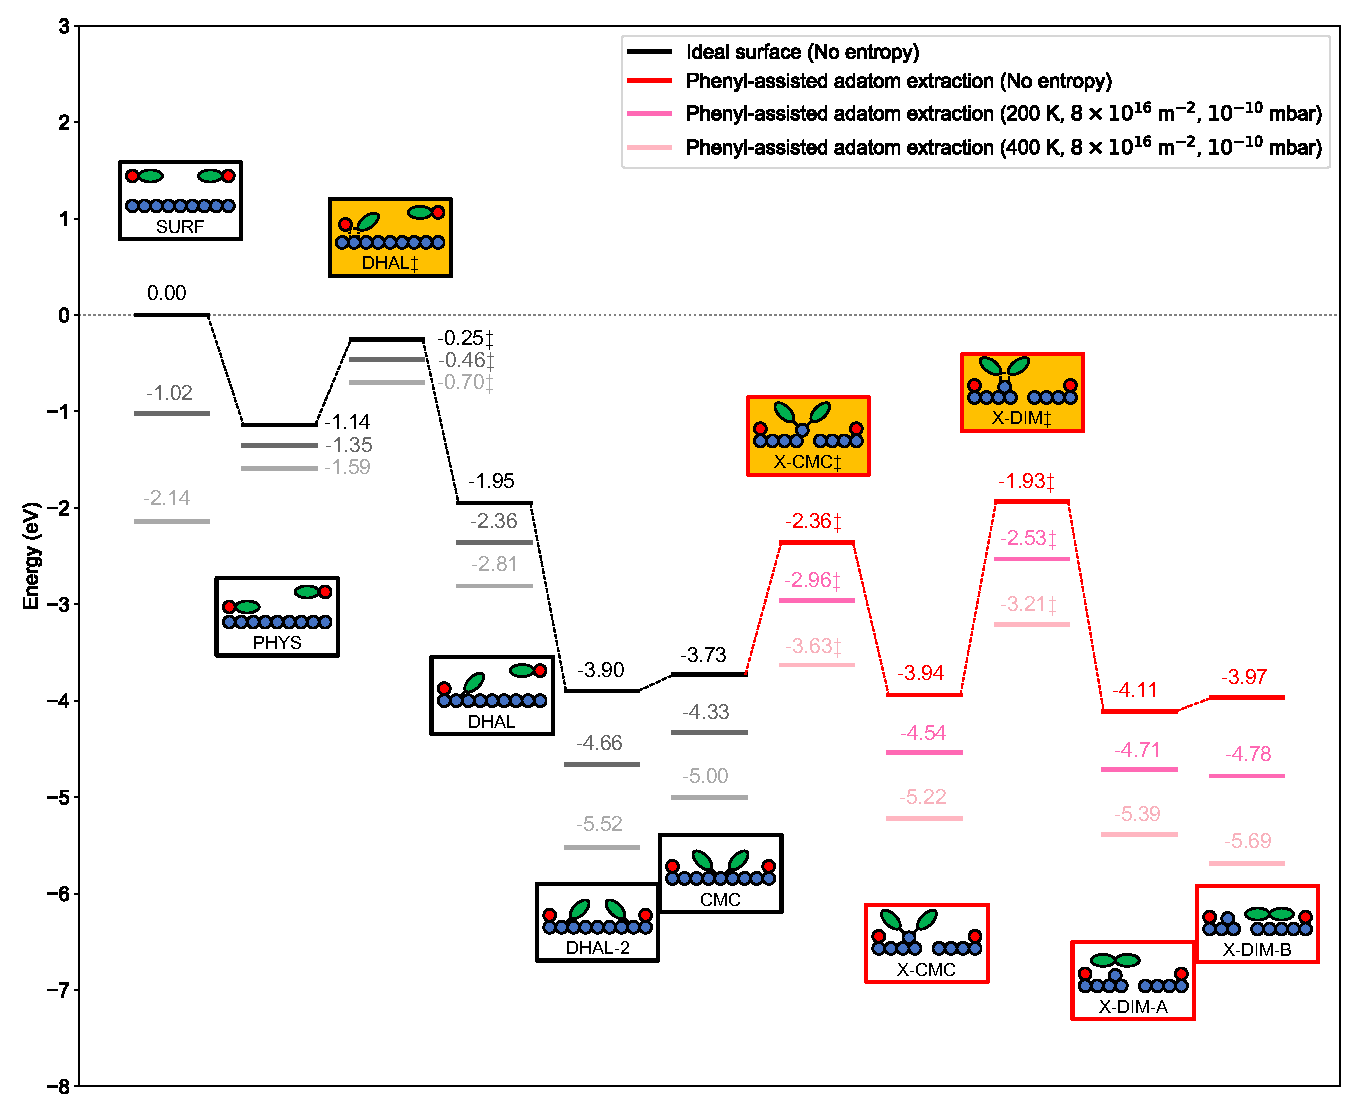
\includegraphics[width=0.96\textwidth]{Fig/Entropy_adatom.pdf}
\caption{Energy profile of the Ullmann reaction of bromobenzene on Cu(111) after applying entropy effects following phenyl-assisted adatom extraction pathway. Levels shown with red color are states without additional entropy-related functions, whereas the hotpink and lightpink are states at a experimental pressure and molecular concentration conditions with different temperature, respectively.whereas the hotpink states are with a entropy correction at \SI{200}{\kelvin} temperature and lightpink states are at \SI{400}{\kelvin} temperature. The pressure and molecule concentration are the same as in Fig.~\ref{fig:entropy_ideal}} 
\label{fig:entropy_adatom}
\end{figure*}



\bibliographystyle{achemso}
\bibliography{references}

\end{document}








